\chapter{Asking Las Vegas Millionaires How They Got Rich!}

This School of Hard Knocks field interview, curated by LazyingArt LLC, does not begin at the beginning. It begins with outcomes: a claimed \$30 million loss, a \$6 million investment turning into roughly \$40 million, a \$600 million business sale, and even a dispute about which generation works harder. Only after that teaser splice does Las Vegas appear as the field in which these claims will be tested. We should therefore read the lecture in the order it wants to be heard: first consequence, then setting, then mechanism. No validated mathematical screenshot survives from this lecture, so the equations and diagram below are transcript-led and, where necessary, cautiously reconstructed.

\section{Cold Open, Las Vegas, and the Wealth Field}

The first seconds are a collage of consequences. We hear ruin, gain, and scale before we know who is speaking:
\begin{equation}
L_{\text{Texas claim}} \approx \$30\,\text{million},\qquad
I_{\text{deal}} = \$6\,\text{million},\qquad
\Pi_{\text{deal}} \approx \$40\,\text{million},\qquad
S_{\text{sale}} = \$600\,\text{million}.
\end{equation}
At this point these numbers are not yet explained. They are bait in the good sense: not decoration, but unresolved quantities that the rest of the lecture will gradually assign to particular operators and particular business logics.

Then the host resets the frame. Las Vegas is introduced not simply as atmosphere, but as a searchable wealth field:
\begin{equation}
N_{\text{millionaires}} \approx 60{,}000,\qquad
N_{\text{billionaires}} > 10.
\end{equation}
These counts are not used as audited demographic results. They function instead as the lecture's methodological warrant. If the city is dense with wealth, then moving through casinos, hotels, and restaurants is not random wandering; it is a rough sampling procedure.

The host then narrows the search to Bellagio. The lecture now has three things in place: a city, a search method, and a set of teaser numbers waiting to be resolved.

\section{Bellagio and the Shopping-Center Investor}

At Bellagio the lecture gives us a small false start. A Lamborghini owner rejects the ``have you ever been broke'' premise and offers only a picture of his car. The host moves on. This beat is brief, but it matters: display by itself is not yet doctrine.

The first real case is a shopping-center investor. He answers first in the language of duration:
\begin{equation}
T_{\text{real estate}} = 35\ \text{years}.
\end{equation}
Then, when asked how one gets the money to buy assets, he does not begin with leverage theory or with bravado. He begins with sequence:
\begin{equation}
\text{houses} \;\to\; \text{larger assets} \;\to\; \text{shopping centers}.
\end{equation}
That stepwise ladder is important, because only after it has been stated do the present acquisition numbers arrive:
\begin{equation}
P_{\text{Flamingo}} = \$25\,\text{million},\qquad
P_{\text{north side}} \approx \$20\,\text{million}.
\end{equation}
The lecture's rhythm is deliberate here. We do not start with the large nominal figures. We first hear the smaller rung, then the patient climb, and only then the current scale.

The host next asks about the most money made in a single year, and the investor corrects the frame: not one year, but one deal. That gives us the lecture's first explicit capital-payoff example:
\begin{equation}
I_{\text{deal}} = \$6\,\text{million},\qquad
\Pi_{\text{deal}} \approx \$40\,\text{million}.
\end{equation}
If we interpret ``made \$40 million on a \$6 million investment'' as profit on capital deployed, then the reconstructed multiple is
\begin{align}
M_{\Pi/I}
&\approx \frac{\Pi_{\text{deal}}}{I_{\text{deal}}}
= \frac{40}{6}
\approx 6.7,\\
\text{ROI}
&\approx \left(\frac{\Pi_{\text{deal}}}{I_{\text{deal}}}\right)100\%
\approx 667\%.
\end{align}
This is our notation, not the speaker's, and it should be read cautiously. Still, it captures the scale of the claim that the lecture wants us to hold in mind.

The key move, however, is not the number itself. It is the doctrine that follows. Asked for financial advice, the investor does not give a slogan about abundance. He says to be cautious, because whenever someone is selling something, he is getting rid of a problem. The buyer must therefore learn to read the hidden structure of the asset:
\begin{equation}
\text{seller} \;\Rightarrow\; \text{problem exists},\qquad
\text{buyer} \;\Rightarrow\; \text{identify problem} + \text{design exit}.
\end{equation}
Since no validated board image survives from the lecture, the cleanest way to preserve this logic is with a transcript-derived schematic.

\begin{figure}[h]
\centering
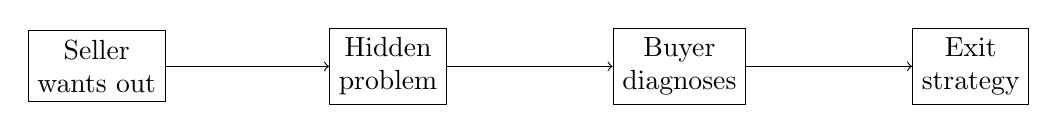
\begin{tikzpicture}
\node[draw, align=center] (a) at (0,0) {Seller\\wants out};
\node[draw, align=center] (b) at (3.7,0) {Hidden\\problem};
\node[draw, align=center] (c) at (7.4,0) {Buyer\\diagnoses};
\node[draw, align=center] (d) at (11.1,0) {Exit\\strategy};
\draw[->] (a) -- (b);
\draw[->] (b) -- (c);
\draw[->] (c) -- (d);
\end{tikzpicture}
\caption{Transcript-derived reconstruction of the shopping-center investor's rule: the gain lies not merely in acquisition, but in identifying the seller's problem and planning the exit.}
\end{figure}

This is the first major conversion in the lecture. We entered with a spectacular payoff number; we are now told what kind of intelligence that number is supposed to represent.

\section{Bank Asymmetry, Age, and the ``Different Game''}

Once the seller-problem doctrine is on the table, the host turns naturally to institutions. What is the lesson about money that banks do not want people to know? The first investor's answer is not a formula about interest. It is a rule about information:
\begin{equation}
\text{operator rule:}\qquad \text{do not tell the bank everything}.
\end{equation}
In other words, the bank is not treated here as a neutral evaluator. It is treated as a counterparty that wants maximal information and maximal claim. The operator's stance is therefore defensive and asymmetrical from the start.

Only after this does the lecture turn to age:
\begin{equation}
a_{\text{older}} = 67,\qquad
a_{\text{host}} = 22,\qquad
\Delta a = 45.
\end{equation}
That difference is not used for decoration. It sets up the next question: whose generation works harder? The investor answers immediately that his own generation does. When pressed, he supports the claim with a concrete self-portrait: at twenty-two he had two jewelry stores, was hustling on the street, wholesaling and retailing, traveling to Italy to buy inventory, and doing all of it on a shoestring. The lecture has moved from commercial intelligence to formation of character.

Now the host steps in with an explicit recap. He says the investor is playing a completely different game. The doctrine is sharpened into a more provocative form:
\begin{equation}
\text{deal size} \uparrow \quad \Rightarrow \quad \text{difficulty} \downarrow
\end{equation}
within the investor's commercial-real-estate frame. The claim is not that every bigger deal is easy. It is that, in this tier of commercial work, size can change the quality of the counterparties, the financing, and the whole structure of execution.

\subsection{Question \& Answer}

\paragraph{Question.} Why can a larger commercial deal be easier rather than harder?

\paragraph{Answer.} Because, in the operator's own frame, scale changes the game before it merely enlarges the number. Larger commercial deals may take longer, but they also bring more professional teams, cleaner financing channels, and counterparties who understand what the asset is. The lecture does not offer this as a universal theorem. It offers it as a rule of one commercial world: above a certain threshold, nominal size and practical difficulty need not move together.

\section{The Apparel Entrepreneur: Brand Horizon, Margin, and the Purchase-Order Trap}

The lecture then changes businesses without abandoning pressure. We leave property and enter apparel, but again the speaker begins not with glamour but with duration and seriousness:
\begin{equation}
T_{\text{apparel}} \approx 10\ \text{years},\qquad
Y_{\text{apparel}} \in \text{seven figures}.
\end{equation}
Before we hear about cost and price, we hear about horizon. This is to be a long-term brand, not a momentary trend. Jay-Z and Ralph Lauren enter not as celebrity garnish, but as a way of distinguishing durable business identity from passing fashion.

Only then does the entrepreneur move to arithmetic. One must know what one is manufacturing and what one is going to sell it for. The natural compact form is
\begin{equation}
m = p - c,
\end{equation}
where \(p\) is selling price, \(c\) is unit production cost, and \(m\) is margin. The lecture never writes this formula down, but it is plainly the economic skeleton of what is being said.

The transcript then becomes somewhat messy in operational detail. The entrepreneur speaks both of overseas manufacturing and of local screen-printing and owned production steps. The most conservative way to preserve the point is directional:
\begin{equation}
c_{\text{printer-owned}} < c_{\text{outsourced}}
\quad \Rightarrow \quad
m_{\text{printer-owned}} > m_{\text{outsourced}}.
\end{equation}
We should not pretend to know more than the transcript securely gives us. The robust point is that controlling more of the production chain can widen margin.

From here the lecture widens outward. Nike, Nordstrom, Macy's, and Tilly's are invoked as signs that he is operating at a business level that, in his Samoan and Polynesian context, has not ordinarily been reached. This is not yet the purchase-order problem; it is the social setting in which that problem becomes sharp.

Then the entrepreneur states the trap directly. A big order can be a curse when the business is not yet capitalized to fulfill it:
\begin{equation}
PO_{\text{Nordstrom}} \approx 100\ \text{racks},\qquad
K_{\text{required}} \approx 50\ \text{racks}.
\end{equation}
If we take the slang in its usual sense, then this would mean
\begin{equation}
PO_{\text{Nordstrom}} \approx \$100{,}000,\qquad
K_{\text{required}} \approx \$50{,}000,
\end{equation}
but that conversion must remain cautious. The more secure mathematical point is the ratio. If both quantities are measured in the same unit, then roughly half the nominal order size must be financed before the revenue arrives:
\begin{equation}
\frac{K_{\text{required}}}{PO_{\text{Nordstrom}}}
\approx \frac{50}{100}
= 0.5.
\end{equation}
So the lecture's real claim is not merely that a big order is good, but that success can arrive in a form that exposes structural unreadiness:
\begin{equation}
\text{large order} \not\Rightarrow \text{capacity to fulfill},\qquad
K_{\text{required}} > 0 \text{ before revenue arrives}.
\end{equation}

\subsection{Question \& Answer}

\paragraph{Question.} How can a large retail order become a burden instead of a breakthrough?

\paragraph{Answer.} Because the order is future money, whereas fulfillment is present obligation. Production, labor, materials, and timing have to be financed before the check comes back. The lecture therefore treats a purchase order as a test of structure. It proves access to a higher level, but it simultaneously asks whether the entrepreneur has enough cash, enough relationships, and enough operational discipline to survive the opportunity.

\section{Proximity, Relationships, and Value}

After the purchase-order trap, the lecture turns from arithmetic to motive. Asked about the turning point, the entrepreneur answers with fatherhood. His son is present, and the desire is to pass on generational wealth that he himself did not inherit. This matters because it explains why the earlier cost-margin discussion is not treated as technical trivia. The arithmetic serves an inheritance problem.

From there he moves to relationships and physical environment. If the action is not where one comes from, one must go where the action is. The lecture compresses into a very plain but very strong rule:
\begin{equation}
\text{proximity to affluent operators}
\;\Rightarrow\;
\text{relationships and opportunities}.
\end{equation}
His own phrase is even shorter: success is about proximity.

Only after this does the income marker arrive, and even then the entrepreneur declines precision, saying only that he has done seven figures. The order is telling. Proximity and relationship come before boasting.

Finally the host asks what business lesson people will not learn in school. The answer is again relationships. People buy from people they like. The maxim that closes this part of the lecture then sharpens the whole segment into one line:
\begin{equation}
\text{value absent} \;\Rightarrow\; \text{price becomes the issue}.
\end{equation}
Like the earlier real-estate aphorisms, this is not a law of nature. It is a selling doctrine stated in the speaker's own register. But it deserves to be kept because it shows how the lecture moves from community, to proximity, to business relationships, and finally to pricing power.

\section{Sponsor Interruption: Side-Hustle Arithmetic}

The sponsor block is a real interruption, and it should remain one on the page. The host says he has learned that
\begin{equation}
p_{\text{millionaires with side hustle}} = 45\%
\end{equation}
of millionaires in the United States have some form of side hustle. The arithmetic that follows belongs to a different register from the main lecture:
\begin{equation}
\$10 \to \$1000,\qquad
B_{\text{bonus}} = \$50 \text{ on } \$5.
\end{equation}
These numbers are not part of the interview-derived commercial doctrines. They are part of the host's monetized interlude. The important structural point is simply that the lecture briefly widens from entrepreneurship to side-hustle arithmetic before returning to the unresolved teaser material.

\section{The \$600 Million Exit, the Texas Loss, and the Final Commercial Doctrine}

After the interruption, the lecture closes a loop. The biggest teaser figure finally receives its owner and its source:
\begin{equation}
S_{\text{INX}} = \$600\,\text{million}.
\end{equation}
The operator says this came from selling INX to Presidio. The figure is therefore an exit event, not an ordinary operating year, and the lecture makes that distinction immediately once the case is fully opened.

Then the host deliberately reopens the broke-question. The same man says he went broke because the state of Texas refused payment on a contract, invoked sovereign immunity, and cost him
\begin{equation}
L_{\text{Texas claim}} \approx \$30\,\text{million}.
\end{equation}
We should preserve that explicitly as a speaker claim. What matters next is the doctrine that comes from it. He does not linger in grievance. He states a reset rule:
\begin{equation}
\text{loss} \to \text{reset next day} \to \text{new earning cycle}.
\end{equation}
That is the lecture's last major state-transition formula. A catastrophic event is to be put down like a ticket; the next day's earning begins anyway.

From reset the lecture moves to negotiation. If a prospective customer is already too difficult on the front end, he says, then he would fire that customer and move on:
\begin{equation}
\text{front-end friction too high}
\;\Rightarrow\;
\text{fire customer and move on}.
\end{equation}
The explanation is relational. If the beginning is already broken, then the rest of the relationship is unlikely to improve simply because the contract has been signed.

\subsection{Question \& Answer}

\paragraph{Question.} When should we walk away from a customer instead of forcing the sale?

\paragraph{Answer.} In this operator's frame, we walk away when the difficulty is not incidental but structural, when the friction appears before the relationship has even formed. The lecture's suggestion is that early resistance is often diagnostic. Some hard conversations are normal; some are warnings. The business judgment lies in telling the difference and refusing to mortgage the future merely to close the present sale.

Asked what banks do not want people to know, the same operator now gives a numerical complaint:
\begin{align}
r_{\text{funding}} &\approx 0\%,\\
r_{\text{customer}} &\approx 10\%,\\
\Delta r &= r_{\text{customer}} - r_{\text{funding}} \approx 10\%.
\end{align}
Then come fees. This is certainly rhetorical and simplified, but the logic is clear enough: cheap funding, expensive lending, fee extraction, and then a qualification regime that keeps the borrower inside a vicious cycle.

From banking the lecture returns once more to real estate. If one has \$100{,}000 and wants to make money in real estate, what should one buy? The operator rejects the residential frame entirely. He does not buy residential real estate; he buys commercial. And when asked why, he gives the same doctrine we heard earlier in a different voice: larger commercial deals can be easier because professional teams and longer time horizons make proper execution possible. He adds a market marker:
\begin{equation}
N_{\text{empty federal buildings}} = 14{,}000.
\end{equation}
Commercial real estate, he says, is going to be interesting over the next twenty years.

The lecture then ends in a register broader than commerce but not detached from it. Life is not for sure, business is not for sure, relationships are not for sure, health is not for sure. The only certainty, he says, is the vertical line with God. The closing move matters. The lecture does not merely finish with piety; it reframes all the earlier business rules inside a world of deep instability.

\section{Summary}

This lecture teaches by delayed explanation. It begins with numbers detached from names, then justifies Las Vegas as a wealth field, then lets one real-estate investor move from houses to shopping centers, from one-deal payoff to seller-problem diagnosis, from bank opacity to generational work ethic, and from there to the host's summary claim that larger commercial deals can become easier. It then shifts to apparel, where long-term brand, margin control, and working-capital strain are joined to fatherhood, proximity, relationships, and value. After a sponsor interruption built around the side-hustle statistic, the lecture returns to the businessman whose \$600 million exit and claimed \$30 million Texas loss had framed the opening, and closes with reset doctrine, walk-away negotiation, bank-spread critique, commercial selection, and spiritual orientation.

What gives these interviews coherence is not a single grand theory of wealth, but a repeated structure. A number appears first. Then a mechanism is offered that makes the number intelligible. The \$40 million payoff becomes a lesson about reading the seller's problem. The large apparel order becomes a lesson about pre-revenue financing strain. The \$600 million exit becomes a lesson about loss, reset, and institutional asymmetry. If we preserve that rhythm from anecdote, to quantity, to mechanism, then the chapter stays faithful to the lecture as it actually unfolds.